%%%%%%%%%%%%%%%%%%%%%%%%%%%%%%%%%%%%%%%%%
% Arsclassica Article
% LaTeX Template
% Version 1.1 (1/8/17)
%
% This template has been downloaded from:
% http://www.LaTeXTemplates.com
%
% Original author:
% Lorenzo Pantieri (http://www.lorenzopantieri.net) with extensive modifications by:
% Vel (vel@latextemplates.com)
%
% License:
% CC BY-NC-SA 3.0 (http://creativecommons.org/licenses/by-nc-sa/3.0/)
%
%%%%%%%%%%%%%%%%%%%%%%%%%%%%%%%%%%%%%%%%%

%----------------------------------------------------------------------------------------
%	PACKAGES AND OTHER DOCUMENT CONFIGURATIONS
%----------------------------------------------------------------------------------------


\documentclass[
12pt, % Main document font size
letterpaper, % Paper type, use 'letterpaper' for US Letter paper
oneside, % One page layout (no page indentation)
%twoside, % Two page layout (page indentation for binding and different headers)
headinclude,footinclude, % Extra spacing for the header and footer
BCOR5mm, % Binding correction
]{scrartcl}

\usepackage{authblk}
\input{structure.tex} % Include the structure.tex file which specified the document structure and layout
\usepackage{natbib}
\usepackage[margin=1in]{geometry}
\usepackage{float}

\hyphenation{Fortran hy-phen-ation} % Specify custom hyphenation points in words with dashes where you would like hyphenation to occur, or alternatively, don't put any dashes in a word to stop hyphenation altogether

%----------------------------------------------------------------------------------------
%	TITLE AND AUTHOR(S)
%----------------------------------------------------------------------------------------

\title{\normalfont\spacedallcaps{Batch-effect correction in single-cell RNA sequencing data using JIVE}} % The article title

%\subtitle{Subtitle} % Uncomment to display a subtitle

\author{\spacedlowsmallcaps{Joseph Hastings, Michael J. O'Connell, \& Donghyung Lee*}} % The article author(s) - author affiliations need to be specified in the AUTHOR AFFILIATIONS block

\date{} % An optional date to appear under the author(s)

%----------------------------------------------------------------------------------------

\begin{document}

%----------------------------------------------------------------------------------------
%	HEADERS
%----------------------------------------------------------------------------------------

\renewcommand{\sectionmark}[1]{\markright{\spacedlowsmallcaps{#1}}} % The header for all pages (oneside) or for even pages (twoside)
%\renewcommand{\subsectionmark}[1]{\markright{\thesubsection~#1}} % Uncomment when using the twoside option - this modifies the header on odd pages
\lehead{\mbox{\llap{\small\thepage\kern1em\color{halfgray} \vline}\color{halfgray}\hspace{0.5em}\rightmark\hfil}} % The header style

\pagestyle{scrheadings} % Enable the headers specified in this block

\maketitle % Print the title/author/date block

%----------------------------------------------------------------------------------------
%	ABSTRACT
%----------------------------------------------------------------------------------------

\section*{Abstract} % This section will not appear in the table of contents due to the star (\section*)

Correcting for batch effects is an important step in preprocessing scRNA-seq data prior to analysis. Batch effects are technical artifacts in the data that arise from a multitude of factors: different sequencing technologies, equipment used, or even capture times. These effects are not of interest and obfuscate the true underyling biological signal. In this paper we introduce a novel application of the JIVE method which we use to perform batch-effect correction on multiple scRNA-seq datasets. We employ four evaluation metrics and compare the results against two other tools, Seurat 3 and Harmony, which were developed for this purpose.

%----------------------------------------------------------------------------------------
%	AUTHOR AFFILIATIONS
%----------------------------------------------------------------------------------------

\let\thefootnote\relax\footnotetext{* \textit{Department of Statistics, Miami University}}

%----------------------------------------------------------------------------------------

%----------------------------------------------------------------------------------------
%	TABLE OF CONTENTS & LISTS OF FIGURES AND TABLES
%----------------------------------------------------------------------------------------

\newpage

\setcounter{tocdepth}{2} % Set the depth of the table of contents to show sections and subsections only

\tableofcontents % Print the table of contents

\listoftables % Print the list of tables

\listoffigures % Print the list of figures

\newpage % Start the article content on the second page, remove this if you have a longer abstract that goes onto the second page

%----------------------------------------------------------------------------------------
%	INTRODUCTION
%----------------------------------------------------------------------------------------

\section{Introduction}

\subsection{Single-cell RNA Sequencing}

\paragraph*{}
There have been significant advancements in recent years in single-cell RNA sequencing (scRNA-seq) \citep{luecken2019current}. Single-cell sequencing provides a much more granular look at genomic data when compared to bulk RNA sequencing and allows for the heterogeneity of different cell populations to be preserved.
Multiple sequencing protocols have been developed to capture this information, with prominent examples including CEL-seq2, Drop-seq, MARS-seq, SCRB-seq, Smart-seq, and Smart-seq2 \citet{ziegenhain2017comparative}.
Data consists of count matrix for a given set of genes obtained from a sample of cells. Each row represents a gene and each column is a single cell. The library size for a cell is the sum of all counts across all genes. 
A number within the count matrix represents the number of times that a gene was successfully captured, reverse transcribed, and sequenced for a given cell.
Once the count data are obtained, it is typically normalized to help account for any variability caused by sampling effects within the given sequencing protocol.
An example is counts per million (CPM) normalization where each count is divided by its library size and multiplied by a million.

Another common preprocessing step is the integration of multiple data sets that are obtained from different batches. Unwanted technical variation and differences between count data are known as batch effects \citep{zhang2020combat}. These effects can arise due different sequencing technologies being used or cells being sequenced at different times.
There have been over a dozen methods developed to integrate multiple sources of scRNA-seq data that aim to remove these unwanted batch effects \citep{tran2020benchmark}. Each method produces a "batch-corrected" data set which is then used for downstream analyses.

%------------------------------------------------

\subsection{Batch-Effect Correction Methods}

\subsubsection*{JIVE}

\paragraph*{}
The joint and individual variation explained (JIVE) method \citep{lock2013joint} decomposes two or more biological datasets into three low-rank approximation components: a joint structure among the datasets, individual structures unique to each distinct dataset, and residual noise. If we let $X_1$, $X_2$, ..., $X_k$ be matrices of dimension $p_i \times n$ containing the original datasets, then we have

\begin{align*}
    X_1 &= J_1 + A_1 + \epsilon_1 \\
    X_2 &= J_2 + A_2 + \epsilon_2 \\
    \vdots \\
    X_k &= J_k + A_k + \epsilon_k 
\end{align*}

where $J_i$ denotes the $i^{th}$ joint structure submatrix, $A_i$ denotes the $i^{th}$ individual structure matrix, and $\epsilon_i$ are error matrices with independent entries.

JIVE was created to decompose any set of related data. An example from \citet{lock2013joint} uses gene expression and miRNA data from a set of 234 Glioblastoma Multiforme tumor cells.

The JIVE decomposition estimates the joint and individual structures by minimizing the sum of squared error of the residual matrix. Given an initial estimate for the joint structure, it finds the individual structures to minimize the sum of squared error. Then, given the new individual structures, it finds a new estimate for the joint structure which minimizes the sum of squared error. This process is repeated until a given threshold for convergence is reached. The ranks are estimated by one of two different methods: a permutation test rank selection and a BIC rank selection.

Our main interest is how well this method performs when we apply it in the context of scRNA-seq data batch-effect correction. We expect the joint structure matrix to capture the shared biological structure between scRNA-seq data from different batches and to serve as the batch-corrected dataset.

\subsubsection*{Seurat 3}

\paragraph*{}
The Seurat 3 integration method \citep{stuart2019comprehensive} employs a strategy which anchors diverse datasets together. First, log-normalization is performed on all datasets and expression values are standardized for each gene. A subset of features are selected which exhibit high variance across all datasets. Then an initial dimension reduction method utilizing canonical correlation analysis (CCA) is performed to ensure similarities across datasets are preserved. Canonical correlation vectors (CCV) are then approximated and used to identify K-nearest neighbors (KNN) for each cell within their paired dataset. Mutual nearest neighbors (MNN) are then identified to act as anchors between datasets. These anchors are then filtered, scores, weighted, and used to perform the batch correction. Functions to perform these tasks are available in the Seurat R package.

\subsubsection*{Harmony}

\paragraph*{}
The Harmony integration method \citep{korsunsky2019fast} utilizes principal component analysis (PCA) for dimensionality reduction and then iterates between two algorithms until convergence is reached. The first algorithm clusters cells from multiple batches but ensures that the diversity of batches within each cluster are maximized (i.e., maximum diversity clustering). The second algorithm then uses a mixture model based approach to perform linear batch correction from a given vector of the known batches. The clustering step assigns soft clusters to cells and the correction step uses these clusters to compute new cell embeddings from the previous iteration. Functions to perform these tasks are available in the Harmony R package.

%------------------------------------------------

\subsection{scRNA-seq Datasets}

\paragraph*{}
One simulated dataset and two real scRNA-seq datasets were used to evaluate the performance of the batch correction methods. The two real data sets were acquired using the scRNAseq R package \citep{risso2022scRNAseq}. Principal variance component analysis (PVCA) \citep{li2009principal} was performed for each raw dataset to get an idea of how much variability is attributed to batch labels, cell cluster labels, and random error. PVCA uses principal components from PCA and variance components analysis (VCA) to fit a mixed linear model using factors of interest as random effects to partition estimate and partition total variability in the data.

\subsubsection*{Simulated Data}

\paragraph*{}
The simulated data was created using the Splatter R package \citep{zappia2017splatter} which allows the user to implement a Splat model. The core of the Splat model is a gamma-Poisson distribution which is used to generate a matrix of cell counts for a given number of genes. More than 20 different parameters are available for modifying, including parameters that affect library size, gene means, expression outliers, the presence of batch effects, the size of batch effects, and more. In our dataset, we simulate data for 5000 genes with two batches containing 500 cells each consisting of three different cell types in similar proportions between batches. The frequency of cells in each batch and cell group can be seen in Table~\vref{tab:freq_simdata}.

\begin{table}[ht]
    \caption{Batch and Cell Type Frequency for Simulated Data}
    \centering
    \begin{tabular}{lrrrr}
    \toprule
    Batch Name & Group 1 & Group 2 & Group 3 & Total \\
    \midrule
    Batch1 & $312$ & $136$ & $52$ & $500$ \\
    Batch2 & $294$ & $148$ & $58$ & $500$ \\
    \bottomrule
    \end{tabular}
    \label{tab:freq_simdata}
\end{table}

\subsubsection*{Bacher T-Cell Data}

\paragraph*{}
The Bacher CD4+ T-cell RNA sequencing data \citep{bacher2020low} was obtained from six unexposed and fourteen COVID-19 patients. There are a total of fifteen different batches and six different cell clusters provided. This data was chosen as there are not very large distinctions between batches and clusters, so we wished to see how the methods would perform in this type of scenario. The frequency of cells in each batch and cell group can be seen in Table~\vref{tab:freq_bacher}.

\begin{table}[ht]
    \caption{Batch and Cell Type Frequency for Bacher T-Cell Data}
    \centering
    \begin{tabular}{lrrrrrrr}
    \toprule
    Batch & Central  & Cycling & Cytotoxic & Tfh-like & Transitional & Type-1 IFN  & Total \\
    Name  & Memory   &         &  / Th1    &          & Memory       & signature   &       \\
    \midrule
    14 & $230$ & $1$ &  $76$ & $250$ & $190$ &  $7$ &  $754$ \\
    15 & $239$ & $4$ & $143$ & $425$ & $289$ & $13$ & $1113$ \\
    \bottomrule
    \end{tabular}
    \label{tab:freq_bacher}
\end{table}

\subsubsection*{Zilionis Mouse Lung Data}

\paragraph*{}
The Zilionis mouse lung data \citep{zilionis2019single} analyzed tumor-infiltrating myeloid cells in mouse lung cancers. There are a total of three different batches and seven different cell clusters provided. This data was chosen as there we can see some distinct separation due to a batch effect and the cell clusters are well seperated. The frequency of cells in each batch and cell group can be seen in Table~\vref{tab:freq_zilionis}.

\begin{table}[ht]
    \caption{Batch and Cell Type Frequency for Zilionis Mouse Lung Data}
    \centering
    \begin{tabular}{lrrr}
        \toprule
        Batch Name & B cells & T cells & Total \\
        \midrule
        round1\_20151128 & $641$ & $579$ & $1220$ \\
        round2\_20151217 & $879$ & $434$ & $1313$ \\
        \bottomrule
        \end{tabular}
    \label{tab:freq_zilionis}
\end{table}

In this study, we evaluate the performance of the three batch-effect correction methods above across three scRNA-seq datasets with four different evaluation metrics. We also present multiple improvements to the JIVE computation algorithms which help significantly decrease runtime compared to the current implementation in the R.JIVE R package.

%----------------------------------------------------------------------------------------
%	METHODS
%----------------------------------------------------------------------------------------

\section{Methods}

\subsection{JIVE Algorithm Improvements} \label{jive_improvements}

\paragraph*{}
The JIVE algorithm was implemented into the R.JIVE R package \citep{o2016r} from the original MATLAB code. The base functions provided in this package can take a substantial amount of runtime to get results (taking upwards of 12+ hours depending on data). We improved the speed of these base functions in two main ways: utilizing partial singular value decomposition in the RSpectra R package \citep{qiu2019rspectra} and converting frequently used matrix operations into precompiled C++ code using the Rcpp R package \citep{edelbuettel2011rcpp} and the RcppEigen R package \citep{bates2013fast} which provides access to the Eigen C++ linear algebra library.

\subsubsection*{Partial SVD}

\paragraph*{}
The original R.JIVE code utilizes singular value decompositions (SVD) in many different areas, however only the largest singular values/vectors are used. A full decomposition takes a lot of time and resources to compute and the majority of the output is not used. We switched to using a partial SVD function in the RSpectra R package which returns the largest singular values/vectors of a given matrix.

\subsubsection*{Matrix Multiplication}

\paragraph*{}
The other area in which we made significant improvements was in basic matrix operations. We tested two different functions which implemented C++ code to perform matrix multiplication and compared their performance to the default \%*\% operator in R. One function uses the Armadillo C++ library via the RcppArmadillo R package \citep{eddelbuettel2014rcpparmadillo} and the other uses the Eigen C++ library via the RcppEigen R package. The function using RcppEigen allows us to specify the number of CPU cores to utilize when performing computations.

%------------------------------------------------

\subsection{Batch Correction Evaluation Metrics}

\paragraph*{}
We employed four tools/metrics to evaluate the performance of each of the batch correction methods: visual inspection of t-distributed stochastic neighbor embedding (t-SNE) and uniform manifold approximation and projection (UMAP) dimension reduction plots, k-nearest neighbor batch effect tests (kBET), average silhouette width (ASW), and local inverse Simpson's index (LISI).

For the visual inspections, we expect to see cells from different batches overlapping each other in the plots with distinct cell type clusters. This is indicative of well-mixed (i.e., integrated) batches that preserve cell type heterogeneity.

\subsubsection*{t-Distributed Stochastic Neighbor Embedding}

\paragraph*{}
t-SNE is a non-linear dimension reduction technique \citep{van2008visualizing} that aids in visualizing high-dimensional data by assigning each data point a location in a two or three-dimensional map. It aims to preserve as much of the local structure of the original data as possible while also revealing global structure such as clusters. High dimensional Euclidean distances between points are used to create conditional probabilities of one point picking the other as its neighbor. A similar conditional probability is calculated for a low dimensional representation of the data. The goal of t-SNE is to find a low dimensional (i.e., two or three dimensions) representation that matches the two probabilities as best as possible by minimizing a certain objective function.

\subsubsection*{Uniform Manifold Approximation and Projection}

\paragraph*{}
UMAP is a non-linear dimension reduction technique \citep{mcinnes2018umap} that is based in manifold theory and topological data analysis. It can be separated into two main phases: graph construction and graph layout. In the graph construction phase, a weighted k-nearest neighbor graph is created, transformations are applied to the graph's edges, and asymmetry is dealt with. In short, it ensures that the underlying geometric structure of the data is captured. In the graph layout phase, an objective function is defined that preserves important characteristics present in the k-nearest neighbor graph, and the final UMAP representation is the one which minimizes this function.

\subsubsection*{k-Nearest Neighbor Batch Effect Test}

\paragraph*{}
The kBET metric \citep{buttner2019test} was constructed with the following premise in mind: a subset of a well-mixed dataset with batch-effects removed should have the same distribution of batch labels as the full dataset. A $\chi^2$ -based test is performed for random subsets of a fixed size neighborhood and results from each test (i.e., reject or fail to reject) is averaged over to provide an overall rejection rate. If the rejection rates are low, then we failed to reject most of the tests, and thus the distribution of batch labels in the small neighborhoods were not significantly different from the entire data's distribution of batch labels.

We calculate the rejection rates with neighborhood sizes equal to 5\%, 10\%, 15\%, 20\%, and 25\% of the number of cells in each dataset. We then use the first 30 principal components from the batch-effect corrected datasets to perform the kBET at each neighborhood size. We then calculate the acceptance rate (1 - rejection rate) so that larger values are more desirable. The acceptance rates are then used for comparison across all methods.

\subsubsection*{Average Silhouette Width}

\paragraph*{}
A silhouette is a measure of consistency within clusters of a given dataset \citep{rousseeuw1987silhouettes}. For each data point in a given cluster, we calculate the mean distance between itself and all other points within the same cluster. We also calculate the smallest mean distance between itself and any other data point not in the same cluster. Then a silhouette is the difference of these two values scaled by the largest of the two. A silhouette takes on values between -1 and 1, with values close to 1 indicating that a particular point is appropriately clustered and values close to -1 indicating the opposite. The ASW is the average of all silhouette values which gives an measure of how well-clustered the data are as a whole.

For our purposes, we use the Euclidean distance metric for all calculations. We then subsample our data down to 80\% of the original and use the first 30 principal components from the subsampled batch-effect corrected datasets. We calculate two ASW metrics: ASW batch (the batch labels are the clusters) and ASW cell type (cell type labels are the clusters), and this process is repeated 20 times for each method. ASW batch and ASW cell type results from all methods are separately scaled to be between 0 and 1. We report 1 - ASW batch values so that large values are more desirable. The median values of each of these scores are then used for comparison across all methods.

\subsubsection*{Local Inverse Simpson's Index}

\paragraph*{}
The local inverse Simpon's index \citep{korsunsky2019fast} first builds local Gaussian kernel-based distributions of neighborhoods around each cell. These neighborhoods are then used in conjuction with the inverse Simpon's index to calculate a diversity score which corresponds to the effective number of clusters in a particular cell's neighborhood.

We calculate two LISI metrics: LISI for batch label clusters (iLISI batch) and LISI for cell type clusters (cLISI cell type). Both LISI scores are calculated for each cell in the batch-effect corrected datasets for each method. iLISI and cLISI results from all methods are separately scaled to be between 0 and 1. We report 1 - cLISI cell type so that large values are more desirable. The median values of each of these scores are then used for comparison across all methods.

%----------------------------------------------------------------------------------------
%	RESULTS
%----------------------------------------------------------------------------------------

\section{Results}

\subsection{JIVE Runtime Improvements}

All benchmarks were performed on a laptop with a 3.20 GHz AMD Ryzen 7 processor with 16.0 GB RAM.

\subsubsection*{Partial SVD}

\paragraph*{}
We compared the partial SVD function to the base SVD function that is used in the R.JIVE package. A benchmark was performed on a dataset of size $1000 \times 1000$ generated from a standard normal distribution in which each function call was performed 100 times. The top 1, 5, and 10 singular values/vectors were computed from each function call. The runtimes can be seen in Figure~\vref{fig:partial_svd_benchmark}.

\begin{figure}[H]
    \centering 
    \includegraphics[width=1\columnwidth]{partial_svd_benchmark} 
    \caption[Benchmark for Partial SVD Runtimes]{Benchmark for Partial SVD Runtimes.}
    \label{fig:partial_svd_benchmark} 
\end{figure}

We see that the original functions perform the decompositions in approximately 1.67 seconds on average, while partial SVD functions are performed in 0.08, 0.12, and 0.15 seconds on average. 

\subsubsection*{Matrix Multiplication}

\paragraph*{}
We compared the default matrix multiplication operator \%*\% in R to the implementations in RcppArmadillo and RcppEigen. A benchmark was performed by multiplying two matrices $A$ and $B$ of size $1000 \times 1000$ generated from a standard normal distribution in which each function call was performed 100 times. The performance for each function can be seen in Figure~\vref{fig:mm_benchmark}.

\begin{figure}[H]
    \centering 
    \includegraphics[width=1\columnwidth]{mm_benchmark} 
    \caption[Benchmark for Matrix Multiplication Runtimes]{Benchmark for Matrix Multiplication Runtimes.}
    \label{fig:mm_benchmark} 
\end{figure}

We see the original multiplication operator and the function using RcppArmadillo both averaged just under 0.3 seconds. The next four functions use the RcppEigen utilizing 1, 2, 4, and 8 CPU cores with runtimes of 0.093, 0.047, 0.027, and 0.02 on average, respectively.

\subsubsection*{Overall Improvements}

\paragraph*{}
We compared the runtimes of the original R.JIVE functions to the updated versions which implement the changes in \ref{jive_improvements}. Two matrices $A$ and $B$ of size $200 \times 1000$ were generated from a common joint structure matrix, two unique individual structure matrices, and two residual error matrices generated from a standard normal distribution. A visualization of these datasets can be seen in Figure~\vref{fig:simdata2_orig}.

\begin{figure}[ht]
    \centering 
    \includegraphics[width=1\columnwidth]{simdata2_orig} 
    \caption[Simulation Data for JIVE Benchmarks]{Simulation Data for JIVE Benchmarks.}
    \label{fig:simdata2_orig} 
\end{figure}

The first and second row contain the final matrix in the first column, the joint matrix in the second column, the individual matrix in the third column, and the error matrix in the fourth column for $A$ and $B$, respectively. Matrix values range from between approximately -2 (represented by the color blue) and 2 (represented by the color red). A benchmark was performed in which both the old R.JIVE implementation and the updated version was performed 20 times. We used given ranks of 1 for the joint structure and each individual structure. The runtimes can be seen in Figure~\vref{fig:jive_v2_simdata2_benchmark}.

\begin{figure}[H]
    \centering 
    \includegraphics[width=1\columnwidth]{jive_v2_simdata2_benchmark} 
    \caption[Benchmark for JIVE Improvements]{Benchmark for JIVE Improvements.}
    \label{fig:jive_v2_simdata2_benchmark} 
\end{figure}

We see that the original R.JIVE function performs the decomposition in about 35.8 seconds on average, while the improved function completes it in 4.1 seconds on average.

The two procedures produced close to identical results. Table~\vref{tab:simdata2_variance} shows the proportion of variance attributable to joint structure, individual structure, and residual variance for the two methods.

\begin{table}[ht]
    \caption{Proportion of Variance Attributed to JIVE Decomposition}
    \centering
    \begin{tabular}{lrrclrr}
        \toprule
        Original   & Data1 & Data 2    & $\mid$ & Updated    & Data1 & Data 2 \\
        \midrule
        Joint      & $0.346$ & $0.161$ & $\mid$ & Joint      & $0.346$ & $0.161$ \\
        Individual & $0.400$ & $0.582$ & $\mid$ & Individual & $0.400$ & $0.582$ \\
        Residual   & $0.254$ & $0.256$ & $\mid$ & Residual   & $0.254$ & $0.256$ \\
        \bottomrule
        \end{tabular}
    \label{tab:simdata2_variance}
\end{table}

%------------------------------------------------

\subsection{Simulated Data}

\paragraph*{}
The only preprocessing step performed for the simulated data is a log-normalization. Each cell count is divided by factor proportional to its library size, a pseudo-count of 1 is added (for zero counts), and a log2-transformation is applied. The PVCA plot for the simulated dataset can be seen in Figure~\vref{fig:pvca_simdata}.

\begin{figure}[H]
    \centering 
    \includegraphics[width=1\columnwidth]{pvca_simdata} 
    \caption[PVCA Breakdown for Simulated Data]{PVCA Breakdown for Simulated Data.}
    \label{fig:pvca_simdata} 
\end{figure}

We observe that almost 95\% of the variability within the data is not due to the batch or cell clusters which is consistent with most scRNA-seq data. The t-SNE plots can be seen in Figure~\vref{fig:tsne_simdata} and the UMAP plots can be seen in in Figure~\vref{fig:umap_simdata}.

\begin{figure}[H]
    \centering 
    \includegraphics[width=1\columnwidth]{tsne_simdata} 
    \caption[t-SNE Plots for Simulated Data]{t-SNE Plots for Simulated Data.}
    \label{fig:tsne_simdata}
\end{figure}

\begin{figure}[H]
    \centering 
    \includegraphics[width=1\columnwidth]{umap_simdata} 
    \caption[UMAP Plots for Simulated Data]{UMAP Plots for Simulated Data.}
    \label{fig:umap_simdata} 
\end{figure}

The top half of each plot has cells colored by batch label and the bottom half has cells colored by their respective cell type/cluster label. We can see that each method has the batches overlapping while the cell clusters are still preserved and distinct from one another. In contrast, the raw plots show some clear seperation between batches. The numeric evaluation metrics can be seen in Figure~\vref{fig:metrics_simdata}.

\begin{figure}[H]
    \centering 
    \includegraphics[width=1\columnwidth]{metrics_simdata} 
    \caption[Metrics for Simulated Data]{(A) kBET results, (B) ASW results, and (C) LISI results for Simulated Data.}
    \label{fig:metrics_simdata} 
\end{figure}

The best performing method for the kBET metric is Harmony followed by closely JIVE. Seurat surprisingly performed worse than the raw data. JIVE and Harmony performed well for the ASW batch metric, closely followed by Seurat. However, Seurat outperformed all methods with regards to the ASW cell type metric. This indicates that Seurat was much better at preserving the different cell types within its cell embeddings than JIVE and Harmony, but not able to distinguish between batches. Harmony and JIVE were the top performers on both the iLISI batch and cLISI cell type metrics. Seurat did not do well with regards to iLISI batch, but was serviceable for the cLISI cell type metric. Overall, JIVE and Harmony were the best performing batch-effect correction methods for the simulated data.

%------------------------------------------------

\subsection{Bacher T-Cell Data}

\paragraph*{}
Data preprocessing for the Bacher T-cell data consisted of log-normalization (as described for the simulated data), and the top 2000 genes with the highest variability across all batches were selected for analysis. This was performed using using a standard workflow provided in the Seurat R package. We also chose to select only two of the fifteen total batches. This reduced our total dataset size from $33538 \times 104417$ to $2000 \times 1867$. The PVCA plot for the Bacher T-cell dataset can be seen in Figure~\vref{fig:pvca_bacherdata}.

\begin{figure}[H]
    \centering 
    \includegraphics[width=1\columnwidth]{pvca_bacherdata} 
    \caption[PVCA Breakdown for the Bacher T-Cell Data]{PVCA Breakdown for the Bacher T-Cell Data.}
    \label{fig:pvca_bacherdata} 
\end{figure}

We see more variability attributed to the batch and cell clusters than in our simulated data, with almost 5\% and 10\%, respectively. The t-SNE plots can be seen in Figure~\vref{fig:tsne_bacherdata} and the UMAP plots can be seen in in Figure~\vref{fig:umap_bacherdata}.

\begin{figure}[H]
    \centering 
    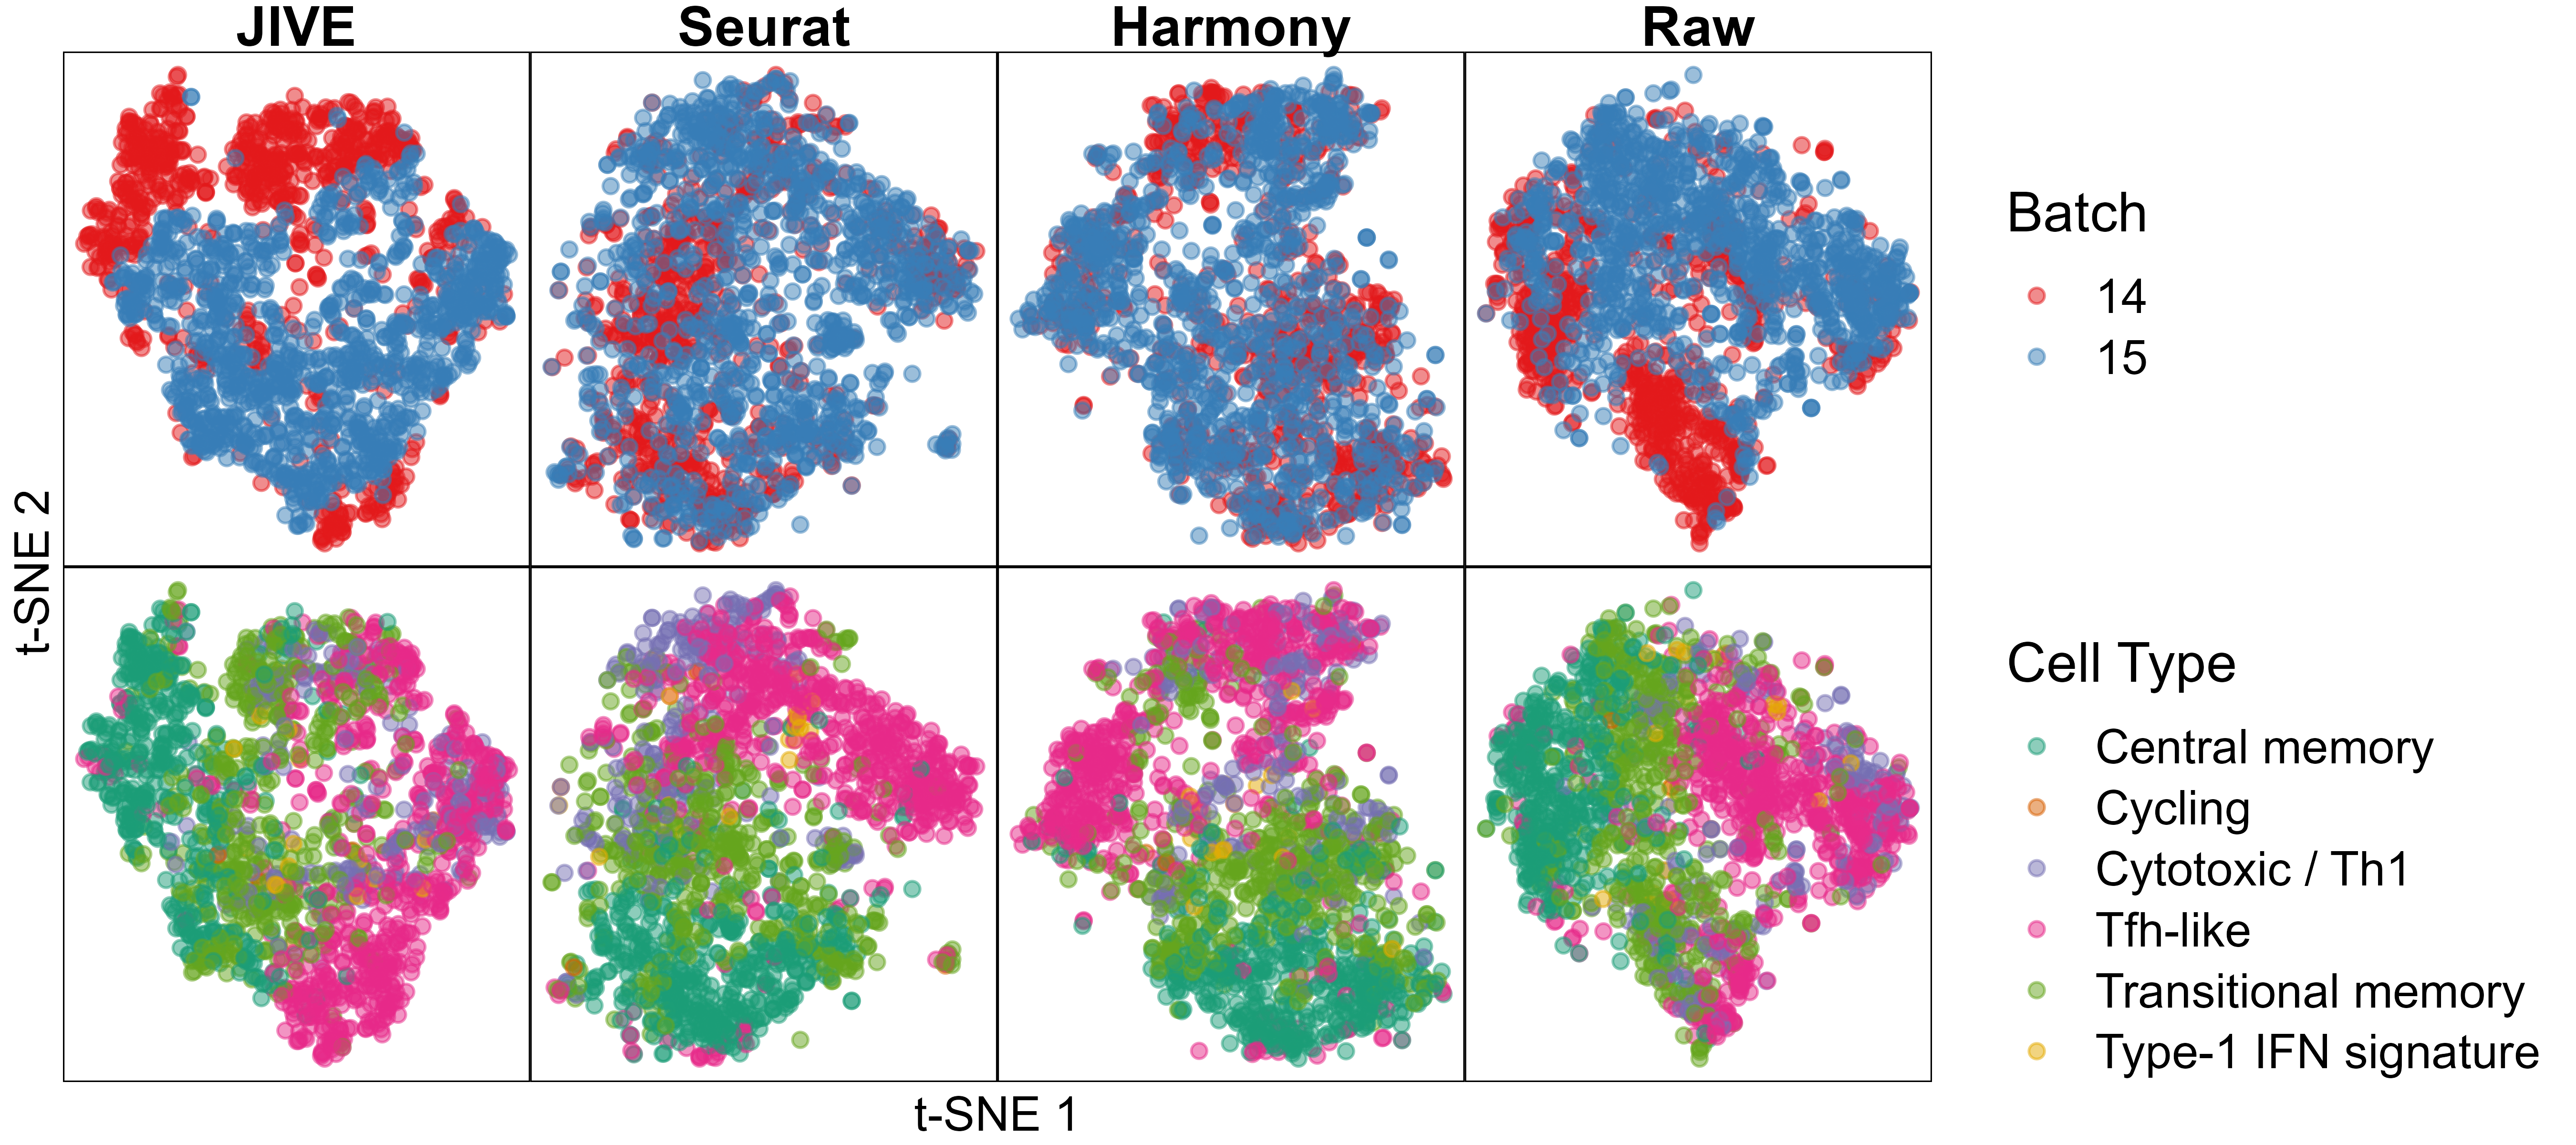
\includegraphics[width=1\columnwidth]{tsne_bacherdata} 
    \caption[t-SNE Plots for the Bacher T-Cell Data]{t-SNE Plots for the Bacher T-Cell Data.}
    \label{fig:tsne_bacherdata}
\end{figure}

\begin{figure}[H]
    \centering 
    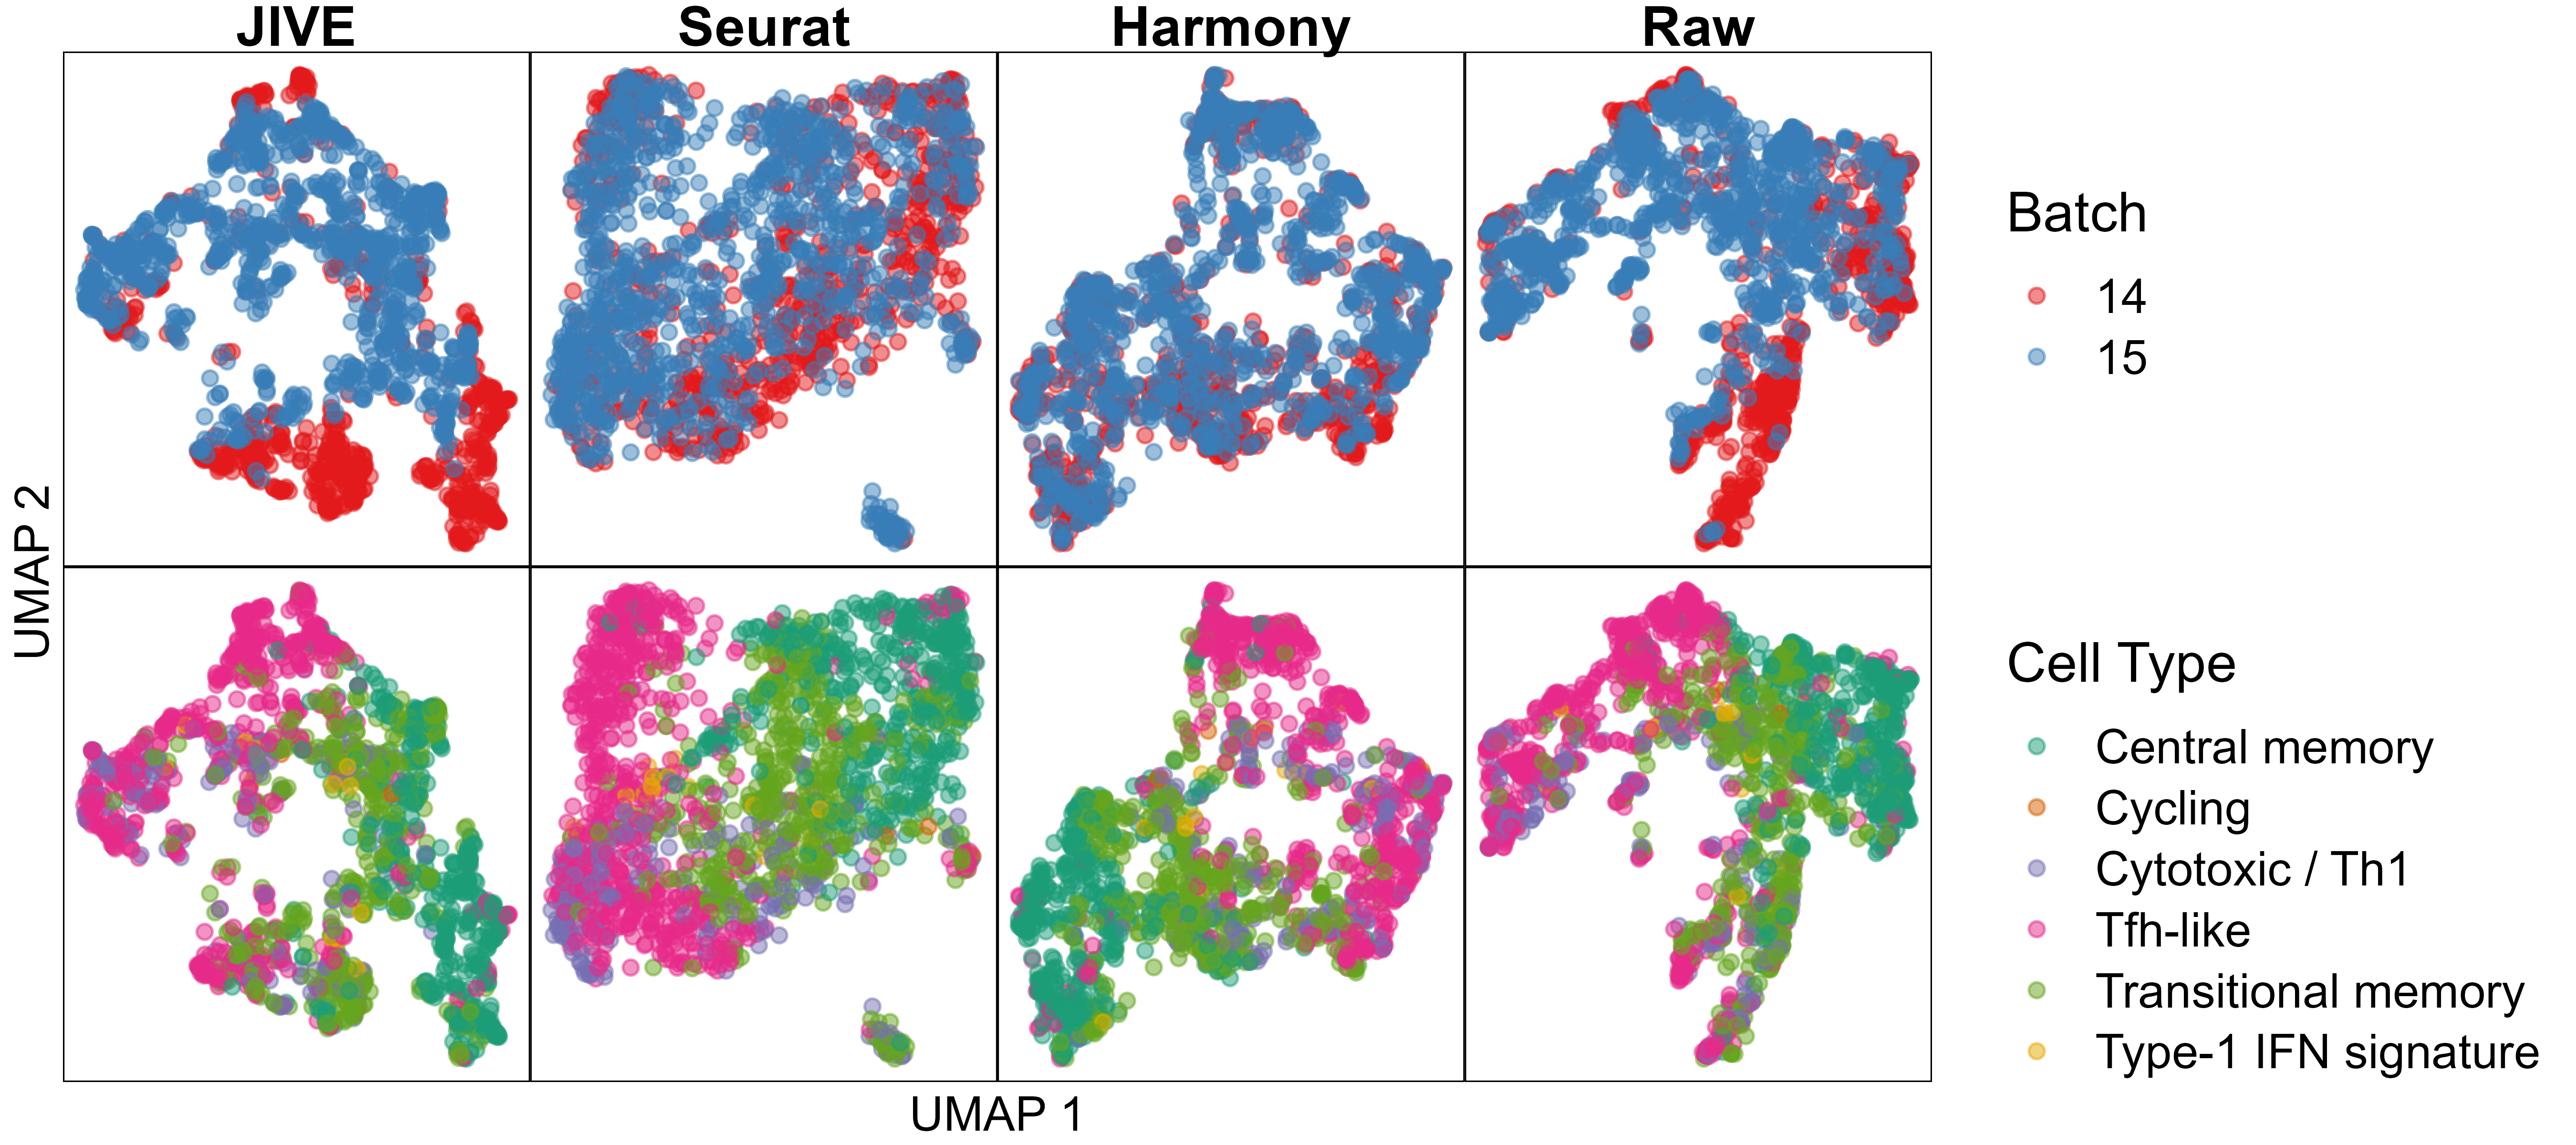
\includegraphics[width=1\columnwidth]{umap_bacherdata} 
    \caption[UMAP Plots for the Bacher T-Cell Data]{UMAP Plots for the Bacher T-Cell Data.}
    \label{fig:umap_bacherdata} 
\end{figure}

We see that Seurat and Harmony both have well-mixed batches in the dimensionality reduction plots, while JIVE does not. The cell clusters look to be well preserved in all three methods. The numeric evaluation metrics can be seen in Figure~\vref{fig:metrics_bacherdata}.

\begin{figure}[H]
    \centering 
    \includegraphics[width=1\columnwidth]{metrics_bacherdata} 
    \caption[Metrics for the Bacher T-Cell Data]{(A) kBET results, (B) ASW results, and (C) LISI results for the Bacher T-Cell Data.}
    \label{fig:metrics_bacherdata} 
\end{figure}

JIVE performs the best with regards to kBET, with JIVE close behind. The acceptance rates for Harmony are just slightly larger than the raw data. Harmony and Seurat both perform best in the ASW metrics, while JIVE only outperforms the raw data with regards to ASW batch and actually performs worse in ASW cell type. Harmony is the clear winner in the LISI metrics followed closely by Seurat. Notably, JIVE performs worse than the raw data in both metrics. It is worth noting that the cLISI cell type is on a much tighter scale than the iLISI batch metric in the plot, so the percieved differences are not as larger as they appear.

%------------------------------------------------

\subsection{Zilionis Mouse Lung Data}

\paragraph*{}
We perform the same preprocessing as described for the Bacher T-cell data, select only two batches, and this time selecting only two cell types/clusters (B-cells and T-cells). This helps to reduce the data dimensions from $28205 \times 17549$ to $2000 \times 2533$. The PVCA plot for the Zilionis Mouse Lung dataset can be seen in Figure~\vref{fig:pvca_zilionisdata}.

\begin{figure}[H]
    \centering 
    \includegraphics[width=1\columnwidth]{pvca_zilionisdata} 
    \caption[PVCA Breakdown for the Zilionis Mouse Lung Data]{PVCA Breakdown for the Zilionis Mouse Lung Data.}
    \label{fig:pvca_zilionisdata} 
\end{figure}

We see a similar breakdown of total variability as the Bacher T-cell data except a bit more is attributed to the cell clusters. The t-SNE plots can be seen in Figure~\vref{fig:tsne_zilionisdata} and the UMAP plots can be seen in in Figure~\vref{fig:umap_zilionisdata}.

\begin{figure}[H]
    \centering 
    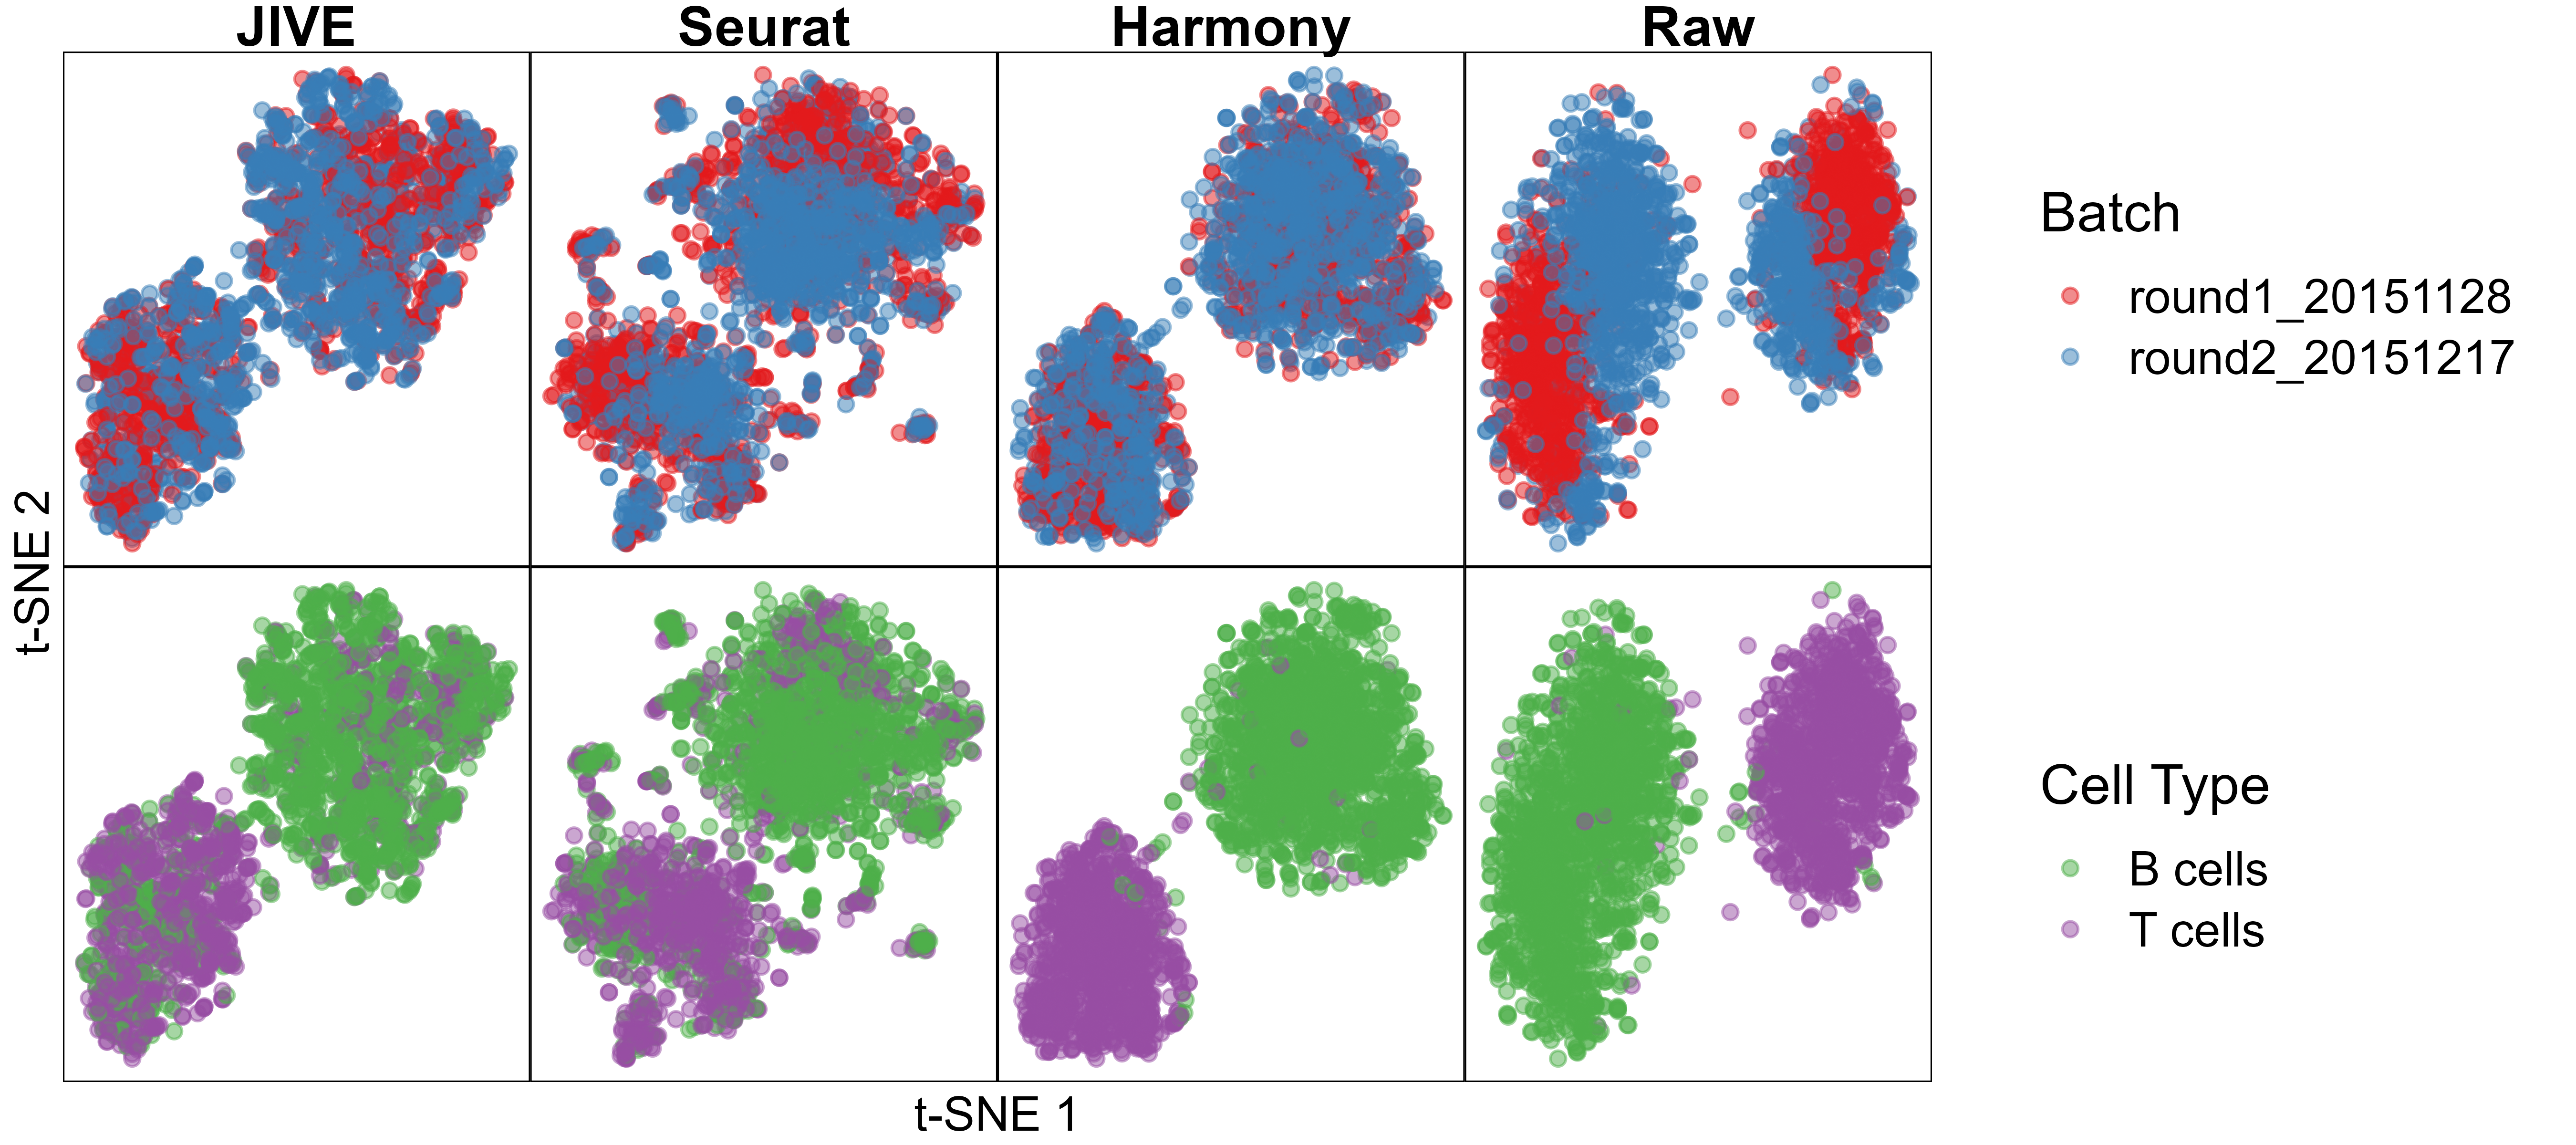
\includegraphics[width=1\columnwidth]{tsne_zilionisdata} 
    \caption[t-SNE Plots for the Zilionis Mouse Lung Data]{t-SNE Plots for the Zilionis Mouse Lung Data.}
    \label{fig:tsne_zilionisdata}
\end{figure}

\begin{figure}[H]
    \centering 
    \includegraphics[width=1\columnwidth]{umap_zilionisdata} 
    \caption[UMAP Plots for the Zilionis Mouse Lung Data]{UMAP Plots for the Zilionis Mouse Lung Data.}
    \label{fig:umap_zilionisdata} 
\end{figure}

We see that each method has well-mixed batches and cell clusters are preserved. It is interesting to note that both JIVE and Seurat produced two distinct clusters that consist of a mix of both cell clusters, while Harmony was able to keep the cell clusters away from each other. The numeric evaluation metrics can be seen in Figure~\vref{fig:metrics_zilionisdata}.

\begin{figure}[H]
    \centering 
    \includegraphics[width=1\columnwidth]{metrics_zilionisdata} 
    \caption[Metrics for the Zilionis Mouse Lung Data]{(A) kBET results, (B) ASW results, and (C) LISI results for the Zilionis Mouse Lung Data.}
    \label{fig:metrics_zilionisdata} 
\end{figure}

We see that all three methods perform similarly at low neighorhood levels. However as the size increases, Seurat drops off dramatically. Harmony seems to perform best at kBET with JIVE close behind. The ASW metric performances are a bit of a mixed bag: each method is better than another at either ASW batch or ASW cell type. Harmony performs best at ASW batch, followed by JIVE and then Seurat. Seurat performs best at ASW cell type, followed by Harmony and then JIVE. JIVE and Harmony are the best performers in the LISI metrics, with JIVE being the best with regards to iLISI batch and Harmony winning out in cLISI cell type. Seurat performs worse than both JIVE and Harmony, and only beats the raw data with regards to iLISI batch.

%----------------------------------------------------------------------------------------
%	DISCUSSION
%----------------------------------------------------------------------------------------

\section{Discussion}



%------------------------------------------------

\subsection{JIVE Algorithm Improvements}

\paragraph*{}
The implementation of a partial SVD function had significant improvements on the overall runtime of the JIVE algorithm. We observed a 95.4\% shorter runtime when estimating one singular value/vector, a 93.1\% shorter runtime when estimating five singular values/vectors, and a 91.0\% shorter runtime when estimating ten singular values/vectors. This is of particular importance because a partial SVD is computed for the joint structure matrix and each individual structure matrix in every iteration of the JIVE estimation algorithm.

Performing matrix multiplication using precompiled C++ code also provided a sizeable decrease in runtime. The difference between the \%*\% operator and the function implemented in RcppArmadillo were neglible. The function implemented in RcppEigen not only provided singificant improvements over the base R operator, but it also allows for the user to specify the amount of CPU cores to utilize during runtime. We observed 67.5\% shorter runtime when using the function with one core, a 83.2\% shorter runtime when using two cores, a 90.6\% shorter runtime when using four cores, and a 92.9\% shorter runtime when using eight cores. Note that using a larger number of available CPU cores does not always provide an increase in speed. Computation on smaller matrices tend to be faster without using multiple cores, but computations on large matrices typically run faster on multiple cores.

\subsection{JIVE Batch-Effect Correction Performance}

\paragraph*{}
In each scRNA-seq dataset, we tested the performance of each batch correction method on their ability mix batches while still preserving the purity of the cell types/clusters. A commonly used method for evaluating batch integration is by visual inspection of dimension reduction plots, with the most common being PCA, t-SNE, or UMAP plots \citep{tran2020benchmark}. This method works well for simple cases like in the simulated data where the batch effects and cell clusters are clearly defined. However, this subjective method tends to become more difficult if there is not clear seperation between batches or when cell types are very similar, as is the case in the Bacher T-cell data. This ambiguity that stems from visual inspection is the reason we employed the use of three numeric evaluation metrics to objectively assess the performance of each method. Note that while objective measurements are useful, we still believe that visual inspection can still provide useful insight during exploratory analysis. Note that none of the metrics simultaneously test both the quality of batch mixing and preservation of cell types, and the development of such a metric would be of great interest.

Overall, we think Harmony performed the best in the simulated data and Zilionis mouse lung data where batch effects were distinct and cell types effets were large. It consistenly performed well on kBET and LISI metrics that take into account the structure of each cell's local neighborhood. The t-SNE and UMAP plots were also consistent with its performance in the numeric metrics. JIVE performed second best with regards to metrics concerning batch mixing, but it struggled greatly with cell type purity metrics. The only dataset where it outperformed the raw data was the cLISI metric in the simulated data. Despite this, it was encouraging to see that JIVE was able keep up with Harmony in both the simulated data and the Zilonis mousel lung data. Seurat performed second best at metrics concerning cell type purity and had its best performance in the nebulous Bacher T-cell data. The increase in neighorhood size did not have much impact on its kBET performance and it did well in both ASW metrics and both LISI metrics. The most interesting result was Seurat's poor kBET performance in the simulated data, which seem to contradict the t-SNE and UMAP plots. 

In conclusion, we were impressed by the performance of JIVE in comparison to two widely used tools, especially as this is just one application of the JIVE decomposition. The significant increase in speed due to the improvements made to the algorithm also make it much more practical to use. 

%----------------------------------------------------------------------------------------
%	BIBLIOGRAPHY
%----------------------------------------------------------------------------------------

\renewcommand{\refname}{\spacedlowsmallcaps{References}} % For modifying the bibliography heading

\bibliographystyle{unsrtnat}
% \bibliographystyle{plainnat}

\bibliography{bibliography.bib} % The file containing the bibliography

\end{document}